\scanpage{6}
Ils correspondent aux sous-groupes \inserted{$H$} de $\mathbb{Z}$, distincts de $\mathbb{Z}$ ($c=\operatorname{card}\mathbb{Z}/H$).....

\uline{Orientation d'un contour} : \deleted{\unsure{Ch.|En.}}

\uline{Prop} Soit\deleted{\unsure{s|x}} $X=(S,A,R)$ un contour \inserted{\deleted{\unsure{strict}}} connexe $\ne\varnothing$.

\noindent\begin{minipage}[t]{.28\linewidth}
\figure{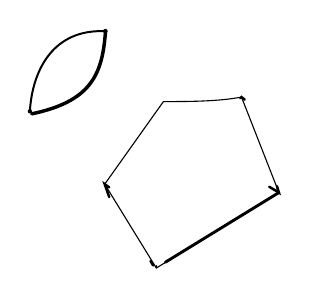
\begin{tikzpicture}[x=.0082cm,y=-.0082cm,line cap=round]
\draw[line width=.72pt] (5,126) .. controls (9,60) and (43,-2) .. (122,2);
\draw[line width=1.25pt] (122,5) .. controls (117,71) and (98,111) .. (8,130);
\fill (5,126) circle[radius=3.4]; \fill (122,2) circle[radius=3.7];
\draw (121,239) -- (212,111) .. controls (249,111) and (297,111) .. (333,104)
  -- (391,252) -- (201,369) -- cycle;
\draw[line width=1.05pt] (215,360) -- (391,252);
\draw[line width=.9pt] (128,244)--(121,239)--(128,259)
  (331,106)--(333,104)--(338,108) (376,243)--(391,252)--(388,242)
  (192,358)--(196,365);
\fill (201,366) circle[radius=1.8];
\end{tikzpicture}}
\end{minipage}\hfill
\begin{minipage}[t]{.68\linewidth}

a) \deleted{Un}\inserted{Soit $g$ un} autom. $g$ de $X$ \deleted{est dit \uline{\unsure{direct}}.}\inserted{Conditions équiv.}

\unsure{\uuline{d'orientation}|\deleted{\uline{d'orientation}}}

$1^{\circ})$ \deleted{si} $\forall s\in S$, $s$ est lié à $gs$

$2^{\circ})$ $\forall a\in A\quad ga$ est lié à $a$

\deleted{\unsure{$\{$|$f$}}

\deleted{\unsure{Déf.|Def.|b)|Si}} On dit que $g$ est une \deleted{\unsure{autom.}} d'\uline{orientation} de $X$.
\end{minipage}

b) Soit $\omega(X)$\inserted{$\subset\operatorname{Aut}(X)$} l'ens des\unsure{.} \deleted{\unsure{autom.} d'}\unsure{orientation|orientations} de $X$

\inserted{Si $g\in\omega(X)$, on a $g^{-1}\in\omega(X)$.}

Alors $\operatorname{card}\omega(X)=2$ \unsure{;|,} \deleted{et si $g\in\unsure{\omega|\omega(X)}$} \inserted{(si $X$ est strict i.e. si $\unsure{c|(}=\operatorname{card}S\ne2$)}, et si $g\in\omega(X)$, on a $\omega(X)=\{g,g^{-1}\}$.

c) \deleted{Soit $\operatorname{Aut}^{+}(X)\subset\operatorname{Aut}(X)$ le ss-grpe de $\operatorname{Aut}X$ formé par les $g\in\operatorname{Aut}X$ tels que $g$ opère \unsure{triv$^{\mathrm{lt}}$|triv$^{\mathrm{t}}$} sur $\omega(X)$ [i.e.}

Considérons $\operatorname{Aut}(X)\unsure{-|\to}\operatorname{Aut}(\omega(X))\simeq\mathbb{Z}/2\mathbb{Z}$.

C'est un hom surjectif, i.e. le noyau $\operatorname{Aut}^{+}(X)$ est un ss-grpe d'indice $2$.

De plus, $\operatorname{Aut}^{+}(X)$ est un groupe cyclique engendré par tt $g\in\omega(X)$.

\uline{Corollaire} $\operatorname{Aut}(X)\simeq\mathbb{Z}/2\mathbb{Z}\cdot\mathbb{Z}/H$ \inserted{(\unsure{produit|produits} $\frac{1}{2}$ direct):}, où $H$ est le ss-grpe de $\mathbb{Z}$ formé des $n\in\mathbb{Z}$ tels que $g^{n}=1$ ($g$ \unsure{etant|étant|etans|étans|dans} une orientation fixé)
% archive sheet number: 5
